
This chapter covers the theoretical background for the research presented in this thesis. Starting with the description of the Standard Model, this chapter will analyze its limits and suggest one possible theoretical extension, supersymmetry. This additional theory can explain some of the phenomena in nature that the Standard Model cannot describe.

\section{The Standard Model of Particle Physics}

The Standard Model of particle physics is a theory that describes three of the forces existing in nature, the electromagnetic, the weak and the strong force and defines the fundamental constituents of matter \cite{Spiesberger:2000ks}. It was developed in the second half of the century as combined theoretical and experimental effort by the research communities from all around the world. Since the first formulation at the beginning of the 1970s the Standard Model successfully predicted all the particles that were discovered later in the century. The most recent particle discoveries such as the top quark (1995), the tauonic neutrino (2000) and finally the Higgs boson (2012) have given further credence to the Standard Model. 

According to this theoretical model the basic constituents of matter are leptons and quarks, which are divided into three families of identical structure. \autoref{table:fermions} shows all the fermions of the Standard Model and their charges, arranged in the three families. Details on the main aspects of this theory are gonna be given in the following sections.

\begin{figure}[tbh!]
	\begin{center}
		
		\begin{tabular}{ | c | c | c | c | c |}
			\hline
			& 1st Generation & 2 Generation & 3rd Generation & charge \\ \hline \hline
			& & & & \\
			leptons & $\left( \begin{array}{c} \nu_{e} \\ e \end{array} \right)_{\text{L}}$ & $\left( \begin{array}{c} \nu_{\mu} \\ \mu \end{array} \right)_{\text{L}}$ & $\left( \begin{array}{c} \nu_{\tau} \\ \tau \end{array} \right)_{\text{L}}$ & \begin{tabular}{@{}c@{}}weak \\ weak, electromagnetic\end{tabular} \\
			& & & & \\
			& $e_{\text{R}}$& $\mu_{\text{R}}$& $\tau_{\text{R}}$& electromagnetic\\ 
			& & & & \\
			\hline
			& & & & \\
			quarks & $\left( \begin{array}{c} u \\ d \end{array} \right)_{\text{L}}$ & $\left( \begin{array}{c} c \\ s \end{array} \right)_{\text{L}}$ & $\left( \begin{array}{c} t \\ b \end{array} \right)_{\text{L}}$ & weak, electromagnetic, strong \\
			& & & & \\
			& $u_{\text{R}}, d_{\text{R}}$& $c_{\text{R}}, s_{\text{R}}$& $t_{\text{R}}, b_{\text{R}}$& electromagnetic, strong\\
			& & & & \\ 
			\hline
			\hline
		\end{tabular}
		\caption{Fermions of the Standard Model and their charges, arranged in the three generations. Only the left-handed fermions interact weakly and are arranged in doublets. The right-handed fermions are singlets. The right-handed neutrinos are not present in this table, as they do not interact with one of the forces of the Standard Model.}
		\label{table:fermions}
	\end{center}
\end{figure}

\subsection{The Higgs Mechanism}
\label{higgs_mechanism}

The discovery of the Higgs boson led to the confirmation of a mechanism that was developed in 1964 to solve the problem of a symmetric Lagrangian with massless particles which did not agreed with experimental evidence. This mechanism works by introducing a new gauge boson and spontaneously breaking symmetry.

The starting point is moving from a global gauge transformation to a point-dependent gauge transformation applied to the minimal Lagrangian $\mathcal{L}$. This requires in addition to the starting complex scalar field $\phi$ also a vectorial field $A_{\mu}$ analog to the electromagnetic field. The resulting Lagrangian is:

\begin{equation}
\mathcal{L} = (D_{\mu}\phi)^{\dagger} D^{\mu}\phi - V (\phi) - \dfrac{1}{4}F_{\mu\nu}F^{\mu\nu}\
\label{eq::lagrangian_min}
\end{equation}

where $V(\phi)$ is the $\phi$ field potential:

\begin{equation}
V(\phi)=\mu^{2}\phi^{\dagger}\phi+\lambda(\phi^{\dagger}\phi)^{2} -\epsilon\phi^{\dagger} -\epsilon^{*}\phi
\end{equation}

$D^{\mu}$ is the covariant derivative:

\begin{equation}
D^{\mu} = \partial^{\mu} - ieA^{\mu},
\end{equation}

and $F^{\mu\nu}$ is the tensor of the vector field $A_{\mu}$:

\begin{equation}
F^{\mu\nu} =\partial^{\nu}A^{\mu} - \partial^{\mu}A^{\nu}.
\end{equation}

where $\epsilon \rightarrow 0$, $\mathcal{L}$ is invariant under gauge transformations:

\begin{equation}
\phi(x) \rightarrow e^{i\alpha(x)}\phi(x); \phi(x)^{\dagger} \rightarrow e ^{-i\alpha(x)}\phi(x)^{\dagger}
\end{equation}

\begin{equation}
A^{\mu} \rightarrow A^{\mu} + \dfrac{1}{e}\partial^{\mu}\alpha(x)
\label{eq::a_tranform}
\end{equation}

where $\alpha(x)$ is an arbitrary function of x and $e$ is a new coupling constant, identical to the electric charge in case $A_{\mu}$ is identified as the electromagnetic field. In order to obtain a stable theory $\lambda > 0$, however $\mu^{2}$ can have two cases depending on the sign choice:
 
1. $\mu^{2} > 0$. The energy minimum is at $\phi = 0$ and $A_{\mu} = 0$. The resulting theory consists of:

\begin{enumerate}
	\item a charged particle and its anti-partner, both with mass $\mu^{2} \neq 0$;
	\item a massless particle with spin 0, similar to the photon.
\end{enumerate}

For small values of $\lambda$ and $e$ the Lagrangian describes the interactions between scalar particles with the electromagnetic field (trough the coupling constant $e$) and their self-interactions (through the couping constant $\lambda$).

2. $\mu^{2} < 0$. The energy minimum is at $A_{\mu} = 0$, so in  case $\epsilon \rightarrow 0$:

\begin{equation}
V(\bar{\phi}) = \text{min }; \quad \bar{\phi}=\eta= 2\lambda +O(\epsilon)
\end{equation}
 
 in order to study the  variations around the minimum $\phi$ is defined as:

\begin{equation}
 \phi=\eta + \dfrac{\sigma_{1}(x) + i\sigma_{2}(x)}{\sqrt{2}} 
\end{equation}

and is used into the minimal Lagrangian \ref{eq::lagrangian_min}.

The particle masses spectrum is obtained from the fields $\sigma_{i}$ and $A_{\mu}$ quadratic terms. In addition, for $\alpha \rightarrow 0$, $\phi$ transforms as:

\begin{equation}
\phi \rightarrow \phi + i\alpha\phi = \eta + \dfrac{\sigma_{1}(x) + i\sigma_{2}(x)}{\sqrt{2}} + i\eta\alpha(x)
\end{equation}

or rather:

\begin{equation}
\sigma_{1}(x) \rightarrow \sigma^{\prime}_{1}(x) = σ_{1}(x); \quad \sigma_{2}(x) \rightarrow \sigma^{\prime}_{2}(x) = \sigma_{2}(x) + \sqrt{2}\eta\alpha(x)
\end{equation}

$A_{\mu}$ transforms following \autoref{eq::a_tranform}. The $\sigma_{2}$ field non-homogeneously transforms by the addition of an $\alpha$ term, arbitrary function of $x$. In case of the given $\sigma_{i}(x)$ and $A_{\mu}$ where:

\begin{equation}
\alpha(x) = -\dfrac{σ\sigma_{2}(x)}{\sqrt{2}\eta}
\end{equation}

resulting in:

\begin{equation}
\sigma^{\prime}_{2}(x) = 0
\label{eq::unitary_gauge}
\end{equation}

the $\sigma_{2}$ filed can be crossed out in case of a gauge symmetry. The gauge identified by \autoref{eq::unitary_gauge} is commonly known as unitary gauge.

\subsection{The bosonic masses}

The starting point is the electroweak Lagrangian $\mathcal{L}_{\text{eW}}$ based on the $\text{SU}(2)_{\text{L}} \oplus \text{U}(1)_{\text{Y}}$ symmetry:

\begin{equation}
\mathcal{L}_{\text{eW}} = \bar{l}i\gamma^{\mu} D_{\mu}l + \bar{e}_{\text{R}}i\gamma^{\mu}D_{\mu}e_{\text{R}} - \dfrac{1}{4}[W_{\mu\nu}W^{\mu\nu} +B_{\mu\nu}B^{\mu\nu}]
\label{eq::lagrangian_ew}
\end{equation}

with the leptonic fields defined as:

\begin{equation}
\binom{(\nu_{e})_{\text{L}}}{e_{\text{L}}}_{\text{Y}=−2} ; \quad (e_{\text{R}})_{\text{Y}=−2}
\label{eq::fields_scheme}
\end{equation}

and the covariant derivatives and tensors defined as:

\begin{equation}
D_{\mu}l = [\partial_{\mu} + igW_{\mu} \dfrac{\tau}{2}  + ig^{\prime}(-\dfrac{1}{2})B_{\mu}]l 
\end{equation}

\begin{equation}
D_{\mu}e_{\text{R}} = [\partial_{\mu} + ig^{\prime}(-1)B_{\mu}]e_{\text{R}}
\end{equation}

\begin{equation}
W_{\mu\nu} =\partial_{\nu}W_{\mu} - \partial_{\mu}W_{\nu} 
\end{equation}

\begin{equation}
B_{\mu\nu} =\partial_{\nu}B_{\mu} - \partial_{\mu}B_{\nu} 
\end{equation}

At this stage the theory describes massless fermions and vectorial fields. The introduction of a scalar field triggers a symmetry breaking while keeping the electromagnetism gauge still intact:

\begin{equation}
\text{SU}(2)_{\text{L}} \oplus \text{U}(1)_{\text{Y}} \rightarrow \text{U}(1)_{\text{em}}
\end{equation}

The optimal choice in order to generate the electron and quarks mass is to choose a $\text{SU}(2)_{\text{L}}$ doublet with $\text{Y} = +1$: 

\begin{equation}
\phi = \binom{(\phi{+})_{\text{L}}}{\phi^{0}}_{\text{Y}=+1}
\label{eq::su2_doublet}
\end{equation}

\begin{equation}
D_{\mu}\phi = [\partial_{\mu} + igW_{\mu} \dfrac{\tau}{2}  + ig^{\prime}(+\dfrac{1}{2})B_{\mu}]\phi 
\end{equation}


with the addition of the fully symmetric Higgs doublet into \autoref{eq::lagrangian_ew} the total Lagrangian becomes:

\begin{equation}
\mathcal{L}_{\text{tot}} = \mathcal{L}_{\text{eW}} + \mathcal{L}_{\phi W}
\end{equation}

where:

\begin{equation}
\mathcal{L}_{\phi W} = (D_{\mu}\phi)^{\dagger} (^{\mu}\phi) - V (\phi);
\label{eq::lagrangian_phiW}
\end{equation}

\begin{equation}
V(\phi) = \mu^{2}\phi^{\dagger}\phi + \lambda(\phi^{\dagger}\phi)^{2}
\end{equation}

Following the example shown in \autoref{higgs_mechanism}, $\phi$ can gain a vacuum expectation term, breaking the symmetry:

\begin{equation}
 \bar{\phi}= < 0|\phi|0 > = \binom{0}{\eta}
 \label{eq::vacuum_expectation}
\end{equation}

where:

\begin{equation}
\eta = \sqrt{\dfrac{-\mu^{2}}{2\lambda}}
\label{eq::eta_value}
\end{equation}

In \autoref{eq::su2_doublet} doublet the electric charge is represented as:

\begin{equation}
Q = 
\begin{pmatrix}
+1 & 0 \\
0 & 0 \\
\end{pmatrix}
\end{equation}

so that the field minimum is invariant under phase transformations associated to $\text{U}_{\text{em}}(1)$:

\begin{equation}
e^{i\alpha Q} \bar{\phi} = 
\begin{pmatrix}
e^{i\alpha} & 0 \\
0 & 1 \\ 
\end{pmatrix}
\binom{0}{\eta}
= \bar{\phi}
\end{equation}

The symmetry breaking given by $\bar{\phi} \neq 0$ gives the scheme \ref{eq::fields_scheme}.
In order to correctly identify all the particles qa definition of the unitary gauge conditions is mandatory. Knowing that every two-dimensional spinor can transform to a spinor with only a real lower component through a point-dependent gauge transformation. Therefore a given $\phi(x)$
can be defined as:

\begin{equation}
\phi(x) = \text{U}(x) \binom{0}{\rho(x)}
\end{equation}

with $\rho(x)$ real and $\text{U}(x)$ as matrix of $ \text{SU}(2)_{\text{L}} \oplus \text{U}(1)_{\text{Y}}$. 

In the previously defined unitary gauge the Lagrangian \ref{eq::lagrangian_phiW} becomes:

\begin{equation}
\begin{array}{l c l}
\mathcal{L}_{\phi W}&=&\dfrac{1}{2} \partial_{\mu} \sigma \partial^{\mu} \sigma - V \left[ \eta + \dfrac{\sigma(x)}{\sqrt{2}}\right] + g^{2} W_{\mu}^{i}(W^{j})^{\mu} \left[ \bar{\phi} \dfrac{\tau_{i}\tau_{j}}{4}\bar{\phi}\right] +\\
&+&(g^{\prime})^{2} \dfrac{1}{4}\eta^{2} B_{\mu} B^{\mu} + 2 gg^{\prime} W^{3}_{\mu} B^{\mu} \left[ \bar{\phi} \dfrac{\tau_{3}}{4} \bar{\phi} \right]
\end{array}
\end{equation}

By using  \autoref{eq::vacuum_expectation} and \autoref{eq::eta_value} along with the Pauli's matrixes properties:

\begin{equation}
\begin{array}{c}
 W_{\mu}^{i}(W^{j})^{\mu} \left[ \bar{\phi} \dfrac{\tau_{i}\tau_{j}}{4}\bar{\phi}\right] = \frac{1}{4}\eta^{2} W_{\mu}W^{\mu} \\

 W^{3}_{\mu} B^{\mu} \left[ \bar{\phi} \dfrac{\tau_{3}}{4} \bar{\phi} \right] = - \dfrac{1}{4} \eta^{2} W^{3}_{\mu}B^{\mu}
 \end{array}
\end{equation}

from the quadratic terms is possible to get the masses value:

\begin{equation}
\begin{array}{c}
W_{\mu}^{i}(W^{j})^{\mu} \left[ \bar{\phi} \dfrac{\tau_{i}\tau_{j}}{4}\bar{\phi}\right] = \frac{1}{4}\eta^{2} W_{\mu}W^{\mu} \\

W^{3}_{\mu} B^{\mu} \left[ \bar{\phi} \dfrac{\tau_{3}}{4} \bar{\phi} \right] = - \dfrac{1}{4} \eta^{2} W^{3}_{\mu}B^{\mu}
\end{array}
\end{equation}

which becomes:

\begin{equation}
\begin{array}{c}
M^{2}  = \dfrac{1}{2} g^{2} \eta^{2}\\
M_{0}^{2}  = \dfrac{1}{2} (g^{\prime})^{2} \eta^{2}\\
M_{03}^{2}  = -\dfrac{1}{2} gg^{\prime} \eta^{2}
\end{array}
\end{equation}

therefore:

\begin{equation}
\mathcal{M} =  \dfrac{1}{2} \eta^{2}
\begin{pmatrix}
 g^{2} & -gg^{\prime} \\
-gg^{\prime} & (g^{\prime})^{2} \\
\end{pmatrix}
\label{eq::matrix_mass}
\end{equation}

in order to allow the existence of a massless photon $det(\mathcal{M}) = 0$. Knowing that the vacuum configuration in invariant to gauge transformation associated to the electric charge is possible to introduce the massive field $Z_{\mu}$ and the electric field $A_{\mu}$ so that:

\begin{equation}
\begin{array}{c}
Z_{\mu} = \cos\theta W^{3}_{\mu} -\sin\theta B_{\mu}\\
A_{\mu} =\sin\theta W^{3}_{\mu} - \cos\theta B_{\mu}

\end{array}
\label{eq::fields_rotation}
\end{equation}

with $\theta$ knows as the electroweak mixing angle. By using the condition that $A_{\mu}$ in the eigen-vector of \autoref{eq::matrix_mass} with a zero eigen-value:

\begin{equation}
0 = 
\begin{pmatrix}
g^{2} & -gg^{\prime} \\
-gg^{\prime} & (g^{\prime})^{2} \\
\end{pmatrix}
\binom{\sin\theta}{\cos\theta}
=
\binom{g^{2}\sin\theta - gg^{\prime}\cos\theta}{-gg^{\prime}\sin\theta + (g^{\prime})^{2}\cos\theta}
\label{eq::matrix_rotation}
\end{equation}

the equation in solved for:

\begin{equation}
\tan\theta = \dfrac{g^{\prime}}{g}
\label{eq::matrix_solution}
\end{equation}

this condition couples the field $A_{\mu}$ defined in \autoref{eq::fields_rotation} with the electron through the electromagnetic current with

\begin{equation}
g\sin\theta = g^{\prime} \cos\prime = e; 
\end{equation}

The theory symmetry breaking made by Weimber and Salam, based on a symmetric Lagrangian, reproduces the masses spectrum and the couplings on the vectorial fields. All those results has been experimentally confirmed.

\subsection{The fermionic masses}

In order to complete the electro-weak theory the calculation of the fermionic masses is mandatory. Starting with the electron mass taken from the $\mathcal{L}_{\text{m}}$ term of the Glashow theory:

\begin{equation}
\mathcal{L}_{\text{m}} = m_{\text{e}}\bar{e}e = m_{\text{e}}(\bar{e}_{\text{L}}e_{\text{R}} + \bar{e}_{\text{R}}e_{\text{L}})
\end{equation}

Another invariant Lagrangian is obtainable by combining $\mathcal{L}_{\text{m}}$ with the Higgs field, which also has the electro-weak iso-spin of $1/2$. Following the symmetry breaking, $\phi$ gains a constant component, which reproduces the Lagrangian  $\mathcal{L}_{\text{m}}$, while the quantum component of $\phi$ gives raise to a new interaction between $\phi$ and the electron. The invariant Lagrangian becomes:

\begin{equation}
\mathcal{L}_{e\phi} = g_{e} (\bar{l}\phi e_{\text{R}} + \bar{e}_{\text{R}}\phi^{\dagger}l)
\end{equation}

The invariant term $\bar{l}\phi$, under spontaneous symmetry breaking, in the unitary gauge becomes:

\begin{equation}
\bar{l}\phi = \bar{\nu}_{\text{L}}\phi^{+} + \bar{e}_{\text{L}}\phi^{0} = \bar{e}_{\text{L}}\left(\eta + \dfrac{\sigma}{\sqrt{2}}\right)
\end{equation}

obtaining:

\begin{equation}
\mathcal{L}_{e\phi} = g_{e}\eta\bar{e}e + g_{e} \dfrac{\sigma}{\sqrt{2}}\bar{e}e = \mathcal{L}_{\text{m}} + \text{interactions}
\end{equation}

resulting in a electron with mass term:

\begin{equation}
m_{\text{e}} = g_{e}\eta
\end{equation}

\subsection{Cabibbo's Theory}

The concept of quark mixing as consequence of the previously introduced symmetry breaking was introduced by Cabibbo \cite{PhysRevLett.10.531}. In this scheme the left-handed fields are are associated to an electroweak doublet and the right-handed ones to singlets:

\begin{equation}
\binom{u}{d}_{\text{L}}; \quad u_{\text{R}}; \quad d_{\text{R}}; \quad s_{\text{L}}; \quad s_{\text{R}}.
\end{equation}

Cabibbo shows that the symmetry breaking leads to a mixing between $d_{\text{L}}$ and $s_{\text{L}}$ leading to a expression of the charged current in the form:

\begin{equation}
J^{1}_{\mu} + i J^{2}_{\mu}= \bar{u}_{\text{L}}\gamma_{\mu} (\cos\theta d_{\text{L}} +\sin\theta s_{\text{L}})
\label{eq::charg_current}
\end{equation}

including a single electroweak parameter, the angle $\theta$ also known as the Cabibbo angle. By the introduction of the triplet:

\begin{equation}
q_{\text{L}} = 
\begin{pmatrix}
u \\
d \\
s \\
\end{pmatrix}
_{\text{L}}
\end{equation}

\autoref{eq::charg_current} becomes:

\begin{equation}
J^{1}_{\mu} + i J^{2}_{\mu} = \bar{q}_{\text{L}}\mathcal{C}\gamma_{\mu}q_{\text{L}} =  \bar{q}_{\text{L}}
\begin{pmatrix}
0 &\cos\theta &\sin\theta \\
0 &0 &0 \\
0 &0 &0\\
\end{pmatrix}
\gamma_{\mu}q_{\text{L}}
\label{eq::charg_current_matrix}
\end{equation}

However the Cabibbo's theory cannot be included in Glashow-Weimber-Salam electroweak theory because \autoref{eq::charg_current_matrix} would lead to a flavor-changing neutral current, in contrast with what shown by experimental data. This current involves the $\mathcal{C}$ commutator which is not diagonal:

\begin{equation}
\left[\mathcal{C}, \mathcal{C}^{\dagger} \right]
=
\begin{pmatrix}
1 &0 &0 \\
0 &\cos^{2}\theta &-\sin\theta \cos\theta \\
0 &-\sin\theta cos\theta &-\sin^{2}\theta\\
\end{pmatrix}
\end{equation}

The neutral current terms in the form of $\bar{d}_{\text{L}}\gamma_{\mu}s_{\text{L}}$ would produce the following decay $K_{\text{L}} \longrightarrow \mu^{+}\mu^{-}$ at the same rate of $K^{+} \longrightarrow \mu^{+}\nu$

\subsection{The Glashow-Iliopoulos-Maiani mechanism}

The flavor-changing neutral current issue was solved in 1970 by S. L. Glashow, J. Iliopoulos e L. Maiani \cite{Glashow:1970gm} by introducing the existence of a fourth quark, named "charm" quark, with the same electroweak quantum numbers of up quark. With the presence of the charm quark the $s_{\text{L}}$ quark goes into a new doublet as follows: 

\begin{equation}
\binom{u}{d}_{\text{L}}; \quad \binom{c}{s}_{\text{L}}; \quad u_{\text{R}}; \quad d_{\text{R}}; \quad c_{\text{R}}; \quad s_{\text{R}}.
\end{equation}

The $\mathcal{C}$ matrix becomes 4 x 4 and the charged weak current becomes:

\begin{equation}
J^{1}_{\mu} + i J^{2}_{\mu} = \bar{q}_{\text{L}} 
\begin{pmatrix}
0 &U_{\text{GIM}} \\
0 &0 \\
\end{pmatrix}
\gamma_{\mu}q_{\text{L}}
\label{eq::cab_current_gim}
\end{equation}

where:

\begin{equation}
U_{\text{GIM}} =
\begin{pmatrix}
\cos\theta &\sin\theta \\
-\sin\theta &\cos\theta \\
\end{pmatrix}
\end{equation}

Given the $U_{\text{GIM}}$ unitarity, the neutral current now becomes:

\begin{equation}
	\begin{array}{l c l}
		J^{3}_{\mu} = \bar{q}_{\text{L}}\left[\mathcal{C}, \mathcal{C}^{\dagger} \right]\gamma_{\mu}q_{\text{L}} = \\
		\bar{q}_{\text{L}}
		\begin{pmatrix}
			U_{\text{GIM}}U_{\text{GIM}}^{\dagger} &0 \\
			0 &-U_{\text{GIM}}^{\dagger}U_{\text{GIM}} \\
		\end{pmatrix}
		\gamma_{\mu}q_{\text{L}} = \bar{q}_{\text{L}}
		\begin{pmatrix}
			1 &0 \\
			0 &-1 \\
		\end{pmatrix}
		\gamma_{\mu}q_{\text{L}}
	\end{array}
\end{equation}

\subsection{CP violation and Kobayashi-Maskawa theory}

After the introduction if the charm quark and the flavor-changing neutral currents suppression, the missing puzzle piece to a fundamental electroweak theory in 1973 was the natural inclusion of CP violation, observed in the neutral mesons K decays since 1964. 
The starting point is demonstrating that a theory with two doublets the $U_{\text{GIM}}$ matrix can always become real under a phase transformation \cite{Glashow:1970gm}. The easiest way to show it starts from the general definition of the Cabibbo's current:

\begin{equation}
J^{\text{C}}_{\mu} = \bar{u}_{\text{L}}\gamma_{\mu}\left( e^{i\alpha} \cos\theta d_{\text{L}} + e^{i\beta}\sin\theta s_{\text{L}}   \right)
\end{equation}

and observe the two phses can be absorbed by the $d_{\text{L}}$ and $s_{\text{L}}$ definitions. At this point the second row of $U_{\text{GIM}}$ is fixed by the condition of being orthonormal to the first row, obtaining:

\begin{equation}
J^{1}_{\mu} + i J^{2}_{\mu} =  \bar{u}_{\text{L}}\gamma_{\mu} \left(\cos\theta d_{\text{L}} +\sin\theta s_{\text{L}}\right) + \bar{c}_{\text{L}}\gamma_{\mu}e^{i\phi} (-\sin\theta d_{\text{L}} + \cos\theta s_{\text{L}})
\end{equation}

is now possible to absorb the phase $e^{i\phi}$ in the field $c_{\text{L}}$ and obtain the real form of the current as shown in \autoref{eq::cab_current_gim}. Given the number of existing left-handed doublets and right handed singlets N M. Kobayashi and T. Maskawa found out that the minimum case where the quark fields can exist with an irreducible phase is at $N = 3$. Given the existence of ad additional doublet the CP violation can now be included in the Weimberg-Salam theory.

\subsection{Masses and Quark mixing}

Once added all the remaining families the general Lagrangian becomes:

\begin{equation}
\mathcal{L}_{ij} = g^{\text{D}}_{ij}\bar{Q}_{i}D_{j} + g^{\text{U}}_{ij}\epsilon_{ab}\bar{U}_{i}Q^{a}_{j}\phi^{b} + \text{h.c.} \quad (i,j = 1,2,3)
\end{equation}

\begin{equation}
\mathcal{L}_{\text{qH}} = \sum_{ij}\mathcal{L}_{ij}
\label{eq::lagrangian_qH}
\end{equation}

where $Q_{i}$ represent the generic left-handed doublet and $U_{i}$ and $D_{i}$ defines the right handed fields of type \textit{up} (u, c, t) and type \textit{down} (d, s, b). The values of the coupling constants $g^{\text{D}}_{ij}$ $g^{\text{U}}_{ij}$ are complex, violating the CP and T symmetry while keeping intact the CPT one.
The quark masses Lagrangian is obtained by using the Higgs field vacuum value in \autoref{eq::lagrangian_qH}:

\begin{equation}
\begin{array}{l c l}
\mathcal{L}_{\text{qm}} = \bar{D}_{\text{L}}M^{\text{d}}D_{\text{R}} + \bar{U}_{\text{R}}M^{\text{u}}U_{\text{L}} + \text{h.c.} \\
(M^{\text{d}})_{ij} = g^{\text{D}}_{ij}\eta; \quad (M^{\text{u}})_{ij} = g^{\text{U}}_{ij}\eta
\end{array}
\end{equation}

where $M^{\text{u}}$ and  $M^{\text{d}}$ are matrices in the doublets family space and they are usually non-diagonal. This introduces a difference between the electroweak base, defined by the quark fields, and the physical base, defined by the fields that diagonalize the mass matrices and directly associated to the physical particles.
The definition of the physical base pass through a decompositions of the $M^{\text{u}}$ and $M^{\text{d}}$ matrices the following way:

\begin{equation}
M^{\text{u}} = W^{\dagger}m_{\text{u}}Z; \quad M^{\text{d}} = U^{\dagger}m_{\text{d}}V
\end{equation}

with $m_u,d$ as positive and diagonal matrices and W, Z, U, V as unitary matrices. The mass Lagrangian is then written:

\begin{equation}
\mathcal{L}_{\text{qm}} = \bar{D}_{\text{L}}U^{\dagger}m_{\text{d}}VD_{\text{R}} + \bar{U}_{\text{R}}W^{\dagger}m_{\text{u}}ZU_{\text{L}} + \text{h.c.}
\end{equation}

The following transformations:

\begin{equation}
U_{\text{R}} \longrightarrow W U_{\text{R}}; \quad D_{\text{R}} \longrightarrow V D_{\text{R}}
\end{equation}

are a redefinition of the electroweak singlets that can be perform in total respect of the electroweak symmetry. A similar redefinition can be also done for the left-handed doublets:

\begin{equation}
Q = \binom{U_{\text{L}}}{D_{\text{L}}} \longrightarrow ZQ
\end{equation}

so the Lagrangian becomes:

\begin{equation}
\begin{array}{l c l}
\mathcal{L}_{\text{qm}} = \bar{D}_{\text{L}}ZU^{\dagger}m_{\text{d}}D_{\text{R}} + \bar{U}_{\text{R}}m_{\text{u}}U_{\text{L}} + \text{h.c.} = \\
= \bar{D}_{\text{L}}U_{\text{CKM}}m_{\text{d}}D_{\text{R}} + \bar{U}_{\text{R}}m_{\text{u}}U_{\text{L}} + \text{h.c.}
\label{eq::Lqm_Uckm}
\end{array}
\end{equation}

The field shown in \autoref{eq::Lqm_Uckm} have still a weak isospin; however in the new base while the U fields have a diagonal mass matrix the D fields are still misaligned. By defining the transformation:

\begin{equation}
\left(D_{\text{ph}}\right)_{\text{L}} = U^{\dagger}_{\text{CKM}}D_{\text{L}}
\end{equation}

or rather:

\begin{equation}
D_{\text{L}} = 
\begin{pmatrix}
d  \\
s  \\
b \\
\end{pmatrix}
_{\text{L}} =
U_{\text{CKM}}\left(D_{\text{ph}}\right)_{\text{L}} = U_{\text{CKM}}
\begin{pmatrix}
d_{\text{ph}}  \\
s_{\text{ph}}  \\
b_{\text{ph}} \\
\end{pmatrix}
_{\text{L}} ;
\end{equation}

\begin{equation}
D_{\text{ph}} = \left(D_{\text{ph}}\right)_{\text{L}} + D_{\text{R}}
\end{equation}

The mass Lagrangian is now finally diagonal:

\begin{equation}
\begin{array}{l c l}
\mathcal{L}_{\text{qm}} = \bar{D}_{\text{L}}ZU^{\dagger}m_{\text{d}}D_{\text{R}} + \bar{U}_{\text{R}}m_{\text{u}}U_{\text{L}} + \text{h.c.} = \\
= \bar{D}_{\text{L}}U_{\text{CKM}}m_{\text{d}}D_{\text{R}} + \bar{U}_{\text{R}}m_{\text{u}}U_{\text{L}} + \text{h.c.} = \\
=  \left(\bar{D}_{\text{ph}}\right)_{\text{L}}m_{\text{d}}D_{\text{R}} + \left(\bar{U}_{\text{ph}}\right)_{\text{R}}m_{\text{u}}\left(U_{\text{ph}}\right)_{\text{L}} + \text{h.c.} = \\
= \bar{D}_{\text{ph}}m_{\text{d}}D_{\text{ph}} + \bar{U}_{\text{ph}}m_{\text{u}}U_{\text{ph}}
\label{eq::Lqm_Uckm_diagonal}
\end{array}
\end{equation}

the matrix $U_{\text{CKM}}$ is indeed the Cabibbo-Kobayashi-Maskawa matrix and it's misalignment breaks the electroweak symmetry.

\subsection{Standard Model limitations}

Over the decades the Standard Model has been successful in predicting particle existence and properties at the electroweak scale. However a few questions remain:

\begin{itemize}
	\item The Standard Model doesn't include gravity, therefore it can't be a complete description of nature;
	\item Although the successful representation of the strong force by the \text{SU}(3), the Standard Model doesn't have the unification of the force coupling constants at the Planck scale.
	\item Astrophysical researches give evidence to the existence of a much greater amount of matter in the universe that can be explained by baryonic matter \cite{deBoer:2005tm}, known also under the name of \textit{dark matter}. The only Standard Model candidate that has properties similar to Dark Matter are neutrinos, however le low rate of neutrino production can't justify the measured dark matter amount;
	\item Neutrinos are considered massless by the Standard Model. Recent experiments showed that neutrinos have masses \cite{Fukuda:1998mi};
	\item In the Standard Model, the quantum corrections to the Higgs mass are quadratically divergent. If the Standard Model is assumed to be valid up to the Planck scale, these corrections are huge compared to the physical Higgs mass.
\end{itemize}

\clearpage

\section{Supersymmetry}

Supersymmetry is one of the most intriguing and fundamental concepts in modern theoretical particle physics. It arises naturally from the combination of the two cornerstones of 20th century physics: quantum mechanics and relativity. Supersymmetry is the unique symmetry that relates the two fundamental kinds of particles: bosons, which act as the carriers of forces, and fermions, which act as the constituents of matter. Supersymmetry transformations are in a sense like the square roots of the coordinate system transformations in special relativity, and consequently supersymmetric quantum field theories have very special, improved properties, compared to ordinary relativistic quantum field theories. If supersymmetry is realized in nature, every fermion in the SM must have a bosonic partner particle and vice versa. No such superpartner particle has been observed so far but there are more and more indications that these particles might show up at the LHC experiments.

\begin{itemize}
	\item supersymmetric lagrangian
\end{itemize}

The most important aspect of superymmetry is the tranformation that turns a bosonic state into a fermionic state, and vice versa. The operator responsible for the transformation Q must be an anti commuting spinor with:

\begin{equation}
Q\left|\text{Bosons}\right> = \left|\text{Fermions}\right>, \quad Q\left|\text{Fermions}\right> = \left|\text{Bosons}\right>. 
\end{equation}

Symmetry is defined as a space-time symmetry given that the Q and $Q^{{+}}$ are able to carry over spin and angular momentum. As a realistic theory with right- and left-handed fermions the transformation generators must fulfill the following commutation and anti-commutation rules:

\begin{equation}
\begin{array}{l c l}
\left\{Q, Q\right\} = P_{\mu}, \\
\left\{Q, Q\right\} = \left\{Q^{\dagger}, Q^{\dagger}\right\} = 0, \\
\left[P_{\mu}, Q\right] = \left[P_{\mu}, Q^{\dagger}\right] = 0,
\end{array}
\end{equation}

where $P_{\mu}$ is the generator of space-time translations. The single-particle states of a supersymmetric theory fall into irreducible representations of the supersymmetry algebra, called supermultiplets. Each of the supermultiplts contains both fermions and bosons, know as eachother \textit{superpartners}. Given the members of the same multiplets $\left|\Omega\right>$ and $\left|\Omega^{\prime}\right>$, $\left|\Omega^{\prime}\right>$ is a combination of the operators Q and $Q^{{+}}$ acting on $\left|\Omega\right>$ and is invariant under space-time translation and rotation transformation. Another important property of the generators  Q and $Q^{{+}}$ is the commutation features with the squared mass operator $-P^{2}$, which translates into the same eigenvalues of the $-P^{2}$ operator shared among of the particles of the supermultiplets, therefore same mass values. Finally the supersimmetric generator transformations commutes with the gauge transformation generators, therefore each of the Standard model particle and its superpartner have  the same electric charges, weak isospin, and color degrees of freedom.
Each supermultiplet also contains an equal number of fermion and boson degrees of freedom \cite{Martin:1997ns}. 

\subsection{Particle content}

\begin{itemize}
	\item ewkino mixing resultin in charginos and neutralinos
	\item multihiggs, explain why there are multiple ones
\end{itemize}

While considering a supersymmetric extension of the Standard Model each of the known fundamental particles belongs to a chiral or gauge multiplets, and has a superpartner with spin differing by $1/2$. The way particles fits into multiplets starts with observing that only chiral supemultiplets can contain fermions for the reason that their left-handed parts transform differently under the gauge group rules than their right-handed parts. All of the Standard Model fermions have those transformation properties, therefore they're members of chiral supermultiplets. On the other hand their superpartners must be spin 0 and not spin 1 vector bosons.

The names for the spin-0 superpartners are constructed by adding the letter \textit{s}, as scalar, at the beginning of the fermion names. So generically they are called squark and sleptons (short form for \textit{scalar quark} and \textit{scalar lepton}). As in the Standard Model each of the two-component Weyl fermions have its own scalar partner. The symbols convention for squarks and sleptons is the same as the corresponding fermion with the addition of the tilde ($\sim$) symbol, e.g. $\tilde{e}$ for the selectron. Is very important to denote that a sfermion given "handedness" does not refer to its helicity, being a spin-0 particle, but to its superparner helicity. A similar nomenclature is applied to smuons and staus: $\tilde{\mu}_{L}$, $\tilde{\mu}_{R}$, $\tilde{\tau}_{L}$, $\tilde{\tau}_{R}$. The Standard Model Neutrinos are always left-handed and their superpartners are generically denoted as $\tilde{\nu}$. The gauge interations of squarks and sleptons are the same as for the corresponding Standard Model fermions; for instance the left handed squarks $\tilde{u_{L}}$ and $\tilde{d_{L}}$ couples with the W bosons, while $\tilde{u_{R}}$ and $\tilde{d_{R}}$ don't.

The Higgs boson is a spin-0 particle so it must reside in a chiral supermultiplet. However with the presence of a single Higgs boson in the supermultiplet the electroweak gauge symmetry would suffer a gauge anomaly, and would be inconsistent as a quantum theory. The conditions for the cancellations of this anomaly include $Tr[T^{2}_{3}Y] = Tr[Y_{3}] = 0$ where T3 and Y are the third component of weak isospin and the weak hypercharge, respectively, in a normalization where the ordinary electric charge is $Q = T_{3} + Y$ . The traces run over all of the left-handed Weyl fermionic degrees of freedom in the theory. In the Standard Model, these conditions are already satisfied by the already known quarks and leptons. The fermionic partner of a Higgs chiral supermultiplet has to be a weak isodoublet with weak hypercharge of $Y = \pm 1/2$. In both case such fermion would give a non-zero contribution to the traces and consequently spoil the anomaly cancellation. This can however be avoided by imposing two higgs supermultiplets, one with each of $Y = \pm1/2$, so that they cancel each other's contribution to the traces out. Another reason to justify the existence of two Higgs boson chiral multiplets is the structure of the supersymmetric theory itself: only the $Y = -1/2 Higgs$ chiral supermultiplet can have the Yukawa couplings necessary to give masses to charge $+2/3$ up-type quarks (up, charm, top), and only a $Y = -1/2$ Higgs can have the Yukawa couplings necessary to give masses to charge $-1/3$ down-type quarks (down, strange, bottom) and to the charged leptons. 

The $\text{SU}(2)_{L}$ scalar fields are defined as $\text{H}_{u}(Y = +1/2)$ and $\text{H}_{d}(Y = -1/2)$. The weak isospin components of $\text{H}_{u}$ with $T_{3} = (1/2, -1/2)$ have electric
charges 1, 0 respectively, and are denoted ($\text{H}^{+}_{u}$, $\text{H}^{0}_{u}$). Similarly, the remaining doublet $\text{H}_{d}$ has $T_{3} = (1/2, -1/2)$ components ($\text{H}^{0}_{d}$, $\text{H}^{-}_{d}$). The Standard Model Higgs is a linear combination of $\text{H}^{0}_{u}$ and $\text{H}^{0}_{d}$. 


We have now found all of the chiral supermultiplets of a minimal phenomenologically viable extension
of the Standard Model. They are summarized in Table 1.1, classified according to their transformation
properties under the Standard Model gauge group SU(3)C × SU(2)L × U(1)Y , which combines
uL, dL and ν, eL degrees of freedom into SU(2)L doublets. Here we follow a standard convention, that
all chiral supermultiplets are defined in terms of left-handed Weyl spinors, so that the conjugates of
the right-handed quarks and leptons (and their superpartners) appear in Table 1.1. This protocol for
defining chiral supermultiplets turns out to be very useful for constructing supersymmetric Lagrangians,
as we will see in section 3. It is also useful to have a symbol for each of the chiral supermultiplets
as a whole; these are indicated in the second column of Table 1.1. Thus, for example, Q stands for
the SU(2)L-doublet chiral supermultiplet containing ueL, uL (with weak isospin component T3 = 1/2),
and edL, dL (with T3 = −1/2), while u stands for the SU(2)L-singlet supermultiplet containing ue
∗
R, u
†
R
.
There are three families for each of the quark and lepton supermultiplets, Table 1.1 lists the first-family
representatives. A family index i = 1, 2, 3 can be affixed to the chiral supermultiplet names (Qi
, ui
, . . .)
when needed, for example (e1, e2, e3) = (e, µ, τ ). The bar on u, d, e fields is part of the name, and does
not denote any kind of conjugation.
The Higgs chiral supermultiplet Hd (containing H0
d
, H
−
d
, He 0
d
, He −
d
) has exactly the same Standard
Model gauge quantum numbers as the left-handed sleptons and leptons Li
, for example (νe, eeL, ν,
eL). Naively, one might therefore suppose that we could have been more economical in our assignment
by taking a neutrino and a Higgs scalar to be superpartners, instead of putting them in separate
supermultiplets. This would amount to the proposal that the Higgs boson and a sneutrino should be the same particle. This attempt played a key role in some of the first attempts to connect supersymmetry to
phenomenology [9], but it is now known to not work. Even ignoring the anomaly cancellation problem
mentioned above, many insoluble phenomenological problems would result, including lepton-number
non-conservation and a mass for at least one of the neutrinos in gross violation of experimental bounds.
Therefore, all of the superpartners of Standard Model particles are really new particles, and cannot be
identified with some other Standard Model state.
The vector bosons of the Standard Model clearly must reside in gauge supermultiplets. Their
fermionic superpartners are generically referred to as gauginos. The SU(3)C color gauge interactions
of QCD are mediated by the gluon, whose spin-1/2 color-octet supersymmetric partner is the gluino. As
usual, a tilde is used to denote the supersymmetric partner of a Standard Model state, so the symbols
for the gluon and gluino are g and ge respectively. The electroweak gauge symmetry SU(2)L × U(1)Y is
associated with spin-1 gauge bosons W+, W0
, W− and B0
, with spin-1/2 superpartners Wf+, Wf0
, Wf−
and Be0
, called winos and bino. After electroweak symmetry breaking, the W0
, B0 gauge eigenstates
mix to give mass eigenstates Z
0 and γ. The corresponding gaugino mixtures of Wf0 and Be0 are called
zino (Ze0
) and photino (γe); if supersymmetry were unbroken, they would be mass eigenstates with
masses mZ and 0. Table 1.2 summarizes the gauge supermultiplets of a minimal supersymmetric
extension of the Standard Model.
The chiral and gauge supermultiplets in Tables 1.1 and 1.2 make up the particle content of the
Minimal Supersymmetric Standard Model (MSSM). The most obvious and interesting feature of this
theory is that none of the superpartners of the Standard Model particles has been discovered as of
this writing. If supersymmetry were unbroken, then there would have to be selectrons eeL and eeR with
masses exactly equal to me = 0.511... MeV. A similar statement applies to each of the other sleptons
and squarks, and there would also have to be a massless gluino and photino. These particles would have
been extraordinarily easy to detect long ago. Clearly, therefore, supersymmetry is a broken symmetry
in the vacuum state chosen by Nature.

\subsection{Motivations}

\begin{itemize}
	\item Dark matter candidate
	\item Higgs corrections \autoref{fig:higgs_loop}
	\item Gravity inclusion
\end{itemize}

\begin{figure}[tbh!]
	\centering
	\begin{tabular}{cc}
		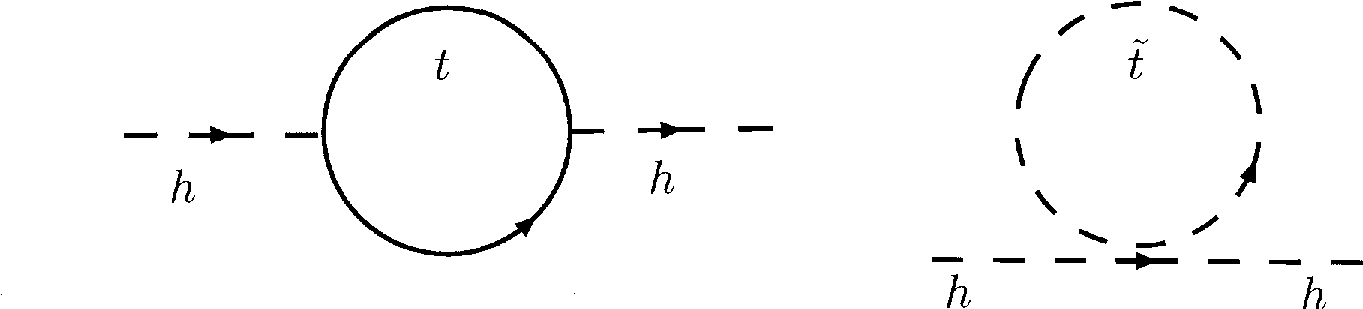
\includegraphics[width=0.75\textwidth]{theory/pics/higgs_loop.png}
	\end{tabular}
	\caption{In SUSY, the correction to Higgs mass by the top quark (L) is inherently cancelled by the contribution from the top quark's supersymmetric partner, the stop (R).}
	\label{fig:higgs_loop}
\end{figure}

\begin{figure}[tbh!]
	\centering
	\begin{tabular}{cc}
		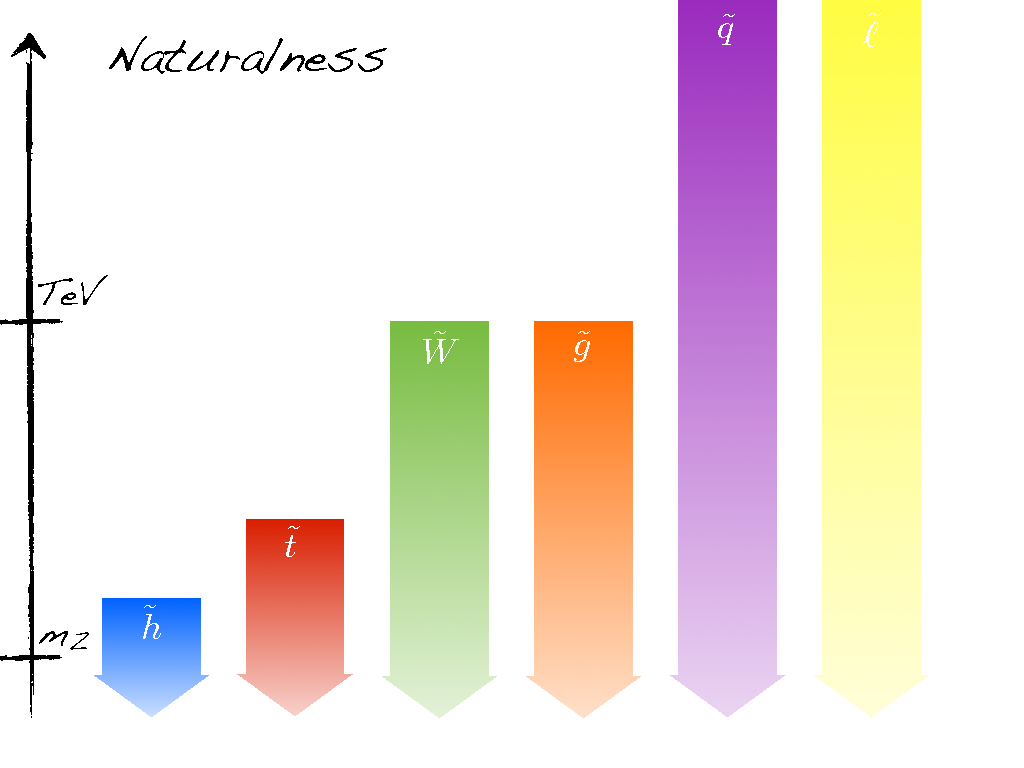
\includegraphics[width=0.75\textwidth]{theory/pics/SUSY_naturalness.png}
	\end{tabular}
	\caption{Cartoon illustration of the mass scales for various sparticles dictated solely by electroweak naturalness with sensitivity parameter $\Delta \lesssim 10$.}
	\label{fig:SUSY_naturalness}
\end{figure}


\begin{figure}[tbh!]
	\centering
	\begin{tabular}{cc}
		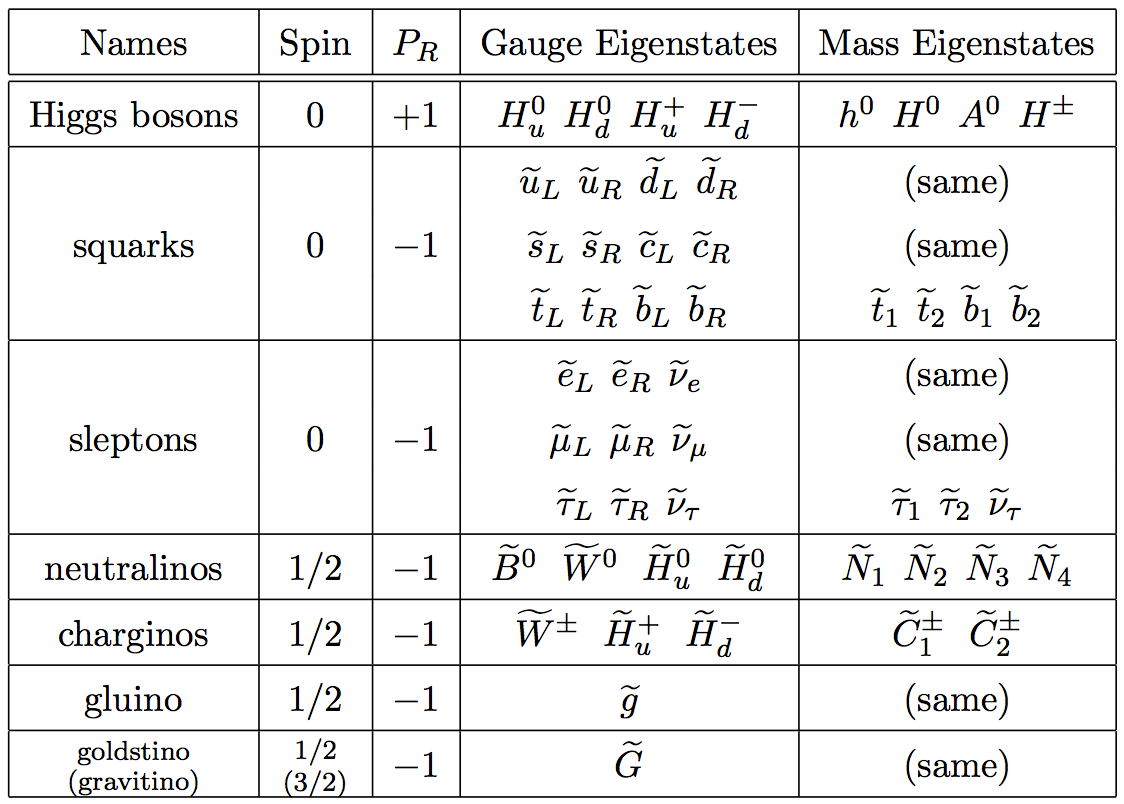
\includegraphics[width=0.75\textwidth]{theory/pics/SUSY_particles_table.png}
	\end{tabular}
	\caption{SUSY particles in MSSM~\protect\cite{Martin:1997ns}}
	\label{fig:SUSY_particles_table}
\end{figure}

\subsection{The MSSM}

\begin{itemize}
	\item R-parity
	\item further assumptions
\end{itemize}


\subsection{SUSY generic signatures at the LHC with charginos and neutralinos}
\begin{itemize}
	\item cascade decays
	\item 3-body decays and mass comfiguration
\end{itemize}


